\begin{abox}
	Electronics
	\end{abox}
\begin{enumerate}
	\item A segment of a circuit is shown in figure $\mathrm{V}_{\mathrm{R}}=5 \mathrm{~V}, \mathrm{~V}_{\mathrm{C}}=4 \sin 2 t$. The voltage $\mathrm{V}_{\mathrm{L}}$ is given by
	\begin{figure}[H]
		\centering
		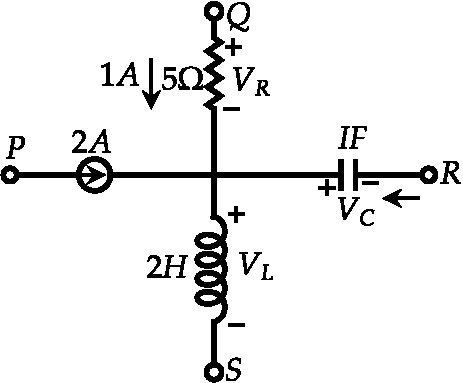
\includegraphics[height=3.5cm,width=4.2cm]{E-A-1}
	\end{figure}
	 \begin{tasks}(2)
		\task[\textbf{a.}]$3-8 \cos 2 t$
		\task[\textbf{b.}]$32 \sin 2 t$
		\task[\textbf{c.}]$16 \sin 2 t$
		\task[\textbf{d.}]  $16 \cos 2 t$
	\end{tasks}
	\item In the circuit of figure, the magnitudes of $\mathrm{V}_{\mathrm{L}}$ and $\mathrm{V}_{\mathrm{C}}$ are twice that of $\mathrm{V}_{\mathrm{R}}$. Given that $f=50 \mathrm{~Hz}$, the inductance of coil is
	\begin{figure}[H]
		\centering
		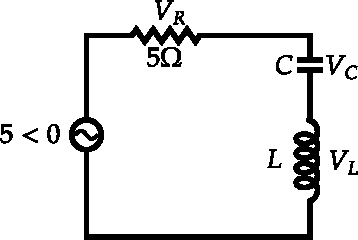
\includegraphics[height=3cm,width=4.5cm]{E-A-2}
		\caption{}
		\label{}
	\end{figure}
	 \begin{tasks}(2)
		\task[\textbf{a.}] $2.14 \mathrm{mH}$
		\task[\textbf{b.}] $5.30 \mathrm{H}$
		\task[\textbf{c.}] $31.8 \mathrm{mH}$
		\task[\textbf{d.}] $1.32 \mathrm{H}$
	\end{tasks}
	\item In the figure value of $R$ is
	\begin{figure}[H]
		\centering
		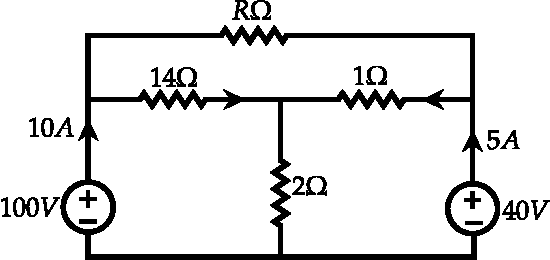
\includegraphics[height=2.6cm,width=5cm]{E-A-3}
		\caption{}
		\label{}
	\end{figure}
	 \begin{tasks}(2)
		\task[\textbf{a.}]$10\Omega$
		\task[\textbf{b.}]$18\Omega$
		\task[\textbf{c.}]$24\Omega$
		\task[\textbf{d.}] $12\Omega$
	\end{tasks}
	\item In figure, the potential difference between points $P$ and $Q$ is
	\begin{figure}[H]
		\centering
		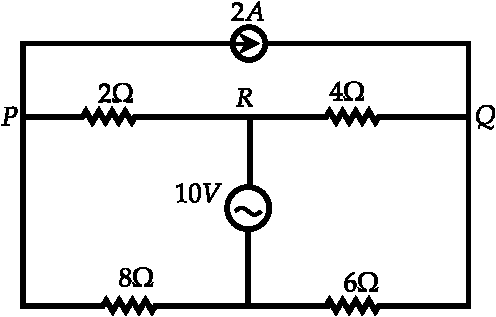
\includegraphics[height=3cm,width=5cm]{E-A-4}
		\caption{}
		\label{}
	\end{figure}
	 \begin{tasks}(2)
		\task[\textbf{a.}]$12V$
		\task[\textbf{b.}]$10V$
		\task[\textbf{c.}]$-6V$
		\task[\textbf{d.}] $8V$
	\end{tasks}
	\item In figure, the value of resistance $R$ in $\Omega$ is
	\begin{figure}[H]
		\centering
		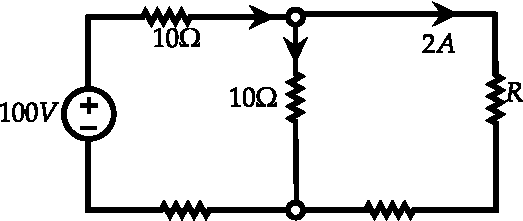
\includegraphics[height=2cm,width=4.5cm]{E-A-5}
		\caption{}
		\label{}
	\end{figure}
	 \begin{tasks}(2)
		\task[\textbf{a.}]10
		\task[\textbf{b.}]20
		\task[\textbf{c.}]30
		\task[\textbf{d.}]40
	\end{tasks}
	\item The RMS value of the voltage $u(t)=3+4 \cos (3 t)$
	 \begin{tasks}(2)
		\task[\textbf{a.}]$\sqrt{17} \mathrm{~V}$
		\task[\textbf{b.}]$5 \mathrm{~V}$
		\task[\textbf{c.}]$7 \mathrm{~V}$
		\task[\textbf{d.}] $(3+2 \sqrt{2}) \mathrm{V}$
	\end{tasks}
	\item Assuming ideal element in the circuit shown below, the voltage $\mathrm{V}_{\mathrm{ab}}$ will be
	\begin{figure}[H]
		\centering
		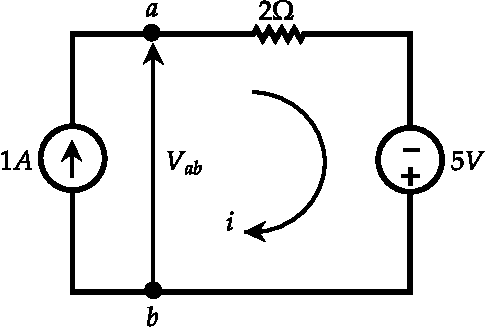
\includegraphics[height=3cm,width=4.5cm]{E-A-6}
	\end{figure}
	 \begin{tasks}(2)
		\task[\textbf{a.}]$-3 \mathrm{~V}$
		\task[\textbf{b.}] $0 \mathrm{~V}$
		\task[\textbf{c.}]$3 \mathrm{~V}$
		\task[\textbf{d.}] $5 \mathrm{~V}$
	\end{tasks}
	\item The current through the $2 \mathrm{k} \Omega$ resistance in the circuit shown is
	\begin{figure}[H]
		\centering
		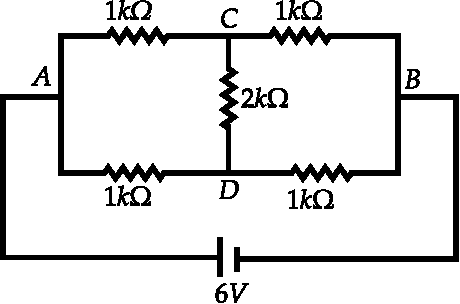
\includegraphics[height=3cm,width=4.5cm]{E-A-7}
		\caption{}
		\label{}
	\end{figure}
	 \begin{tasks}(2)
		\task[\textbf{a.}]$0 \mathrm{~mA}$
		\task[\textbf{b.}]$\operatorname{lm} \mathrm{A}$
		\task[\textbf{c.}]$2 m a$
		\task[\textbf{d.}]  $6 \mathrm{~mA}$
	\end{tasks}
	\item The time constant for the given circuit will be
	\begin{figure}[H]
		\centering
		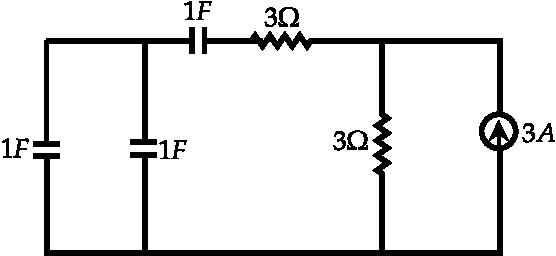
\includegraphics[height=2.5cm,width=5cm]{E-A-8}
	\end{figure}
	 \begin{tasks}(2)
		\task[\textbf{a.}] $1 / \mathrm{gs}$
		\task[\textbf{b.}]$1 / 4 \mathrm{~s}$
		\task[\textbf{c.}] $4 \mathrm{~s}$
		\task[\textbf{d.}] gs
	\end{tasks}
	\item In the circuit given below, the yalue of $R$ required for the transfer of maximum power to the load having a resistance of $3 \Omega$ is
	\begin{figure}[H]
		\centering
		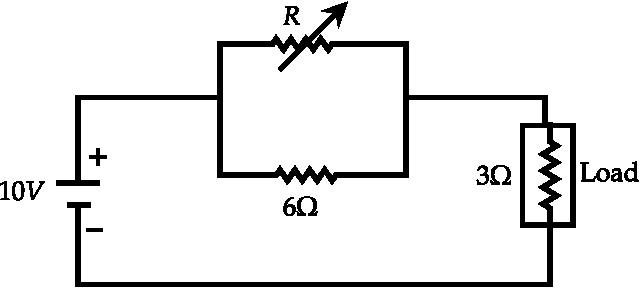
\includegraphics[height=2.5cm,width=5.5cm]{E-A-9}
	\end{figure}
	 \begin{tasks}(2)
		\task[\textbf{a.}]0
		\task[\textbf{b.}]$3\Omega$
		\task[\textbf{c.}]$6\Omega$
		\task[\textbf{d.}] $\infty$
	\end{tasks}
	\item The r.m.s value of the current $i(t)$ in the circuit shown below is 
	\begin{figure}[H]
		\centering
		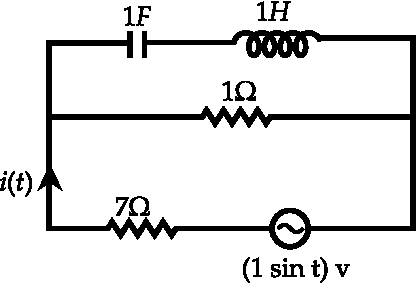
\includegraphics[height=3cm,width=5cm]{E-A-10}
		\caption{}
		\label{}
	\end{figure}
	 \begin{tasks}(2)
		\task[\textbf{a.}]$\frac{1}{2} \mathrm{~A}$
		\task[\textbf{b.}] $\frac{1}{\sqrt{2}} \mathrm{~A}$
		\task[\textbf{c.}]$1 \mathrm{~A}$
		\task[\textbf{d.}]  $\sqrt{2} \mathrm{~A}$
	\end{tasks}
\item In the given figure, the Thevenin's equivalent pair (voltage, impedance), as seen at the terminals $P-Q,$ is given by
\begin{figure}[H]
	\centering
	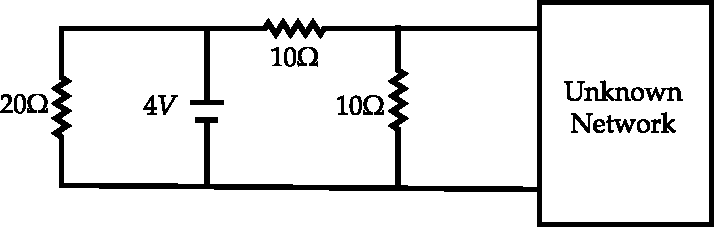
\includegraphics[height=2.3cm,width=6.5cm]{E-A-11}
	\caption{}
	\label{}
\end{figure}
	 \begin{tasks}(2)
		\task[\textbf{a.}]$(2 \mathrm{~V}, 5 \Omega)$
		\task[\textbf{b.}]$(3 \mathrm{~V}, 5 \Omega)$
		\task[\textbf{c.}] $(4 \mathrm{~V}, 5 \Omega)$
		\task[\textbf{d.}] $(2 V, 7.5 \Omega)$
	\end{tasks}
	\item In the circuit shown, the power supplied by the voltage source is
	\begin{figure}[H]
		\centering
		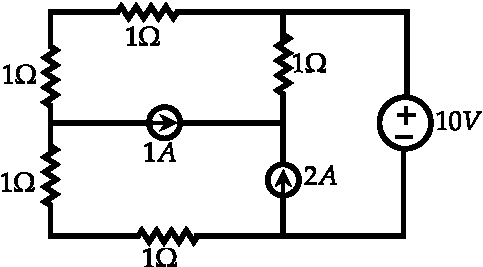
\includegraphics[height=3cm,width=5cm]{E-A-12}
		\caption{}
		\label{}
	\end{figure}
 \begin{tasks}(2)
	\task[\textbf{a.}]0W
	\task[\textbf{b.}]5W
	\task[\textbf{c.}]10W
	\task[\textbf{d.}]100W
\end{tasks}
	\item The voltage $e_{0}$ in the figure is:
	\begin{figure}[H]
		\centering
		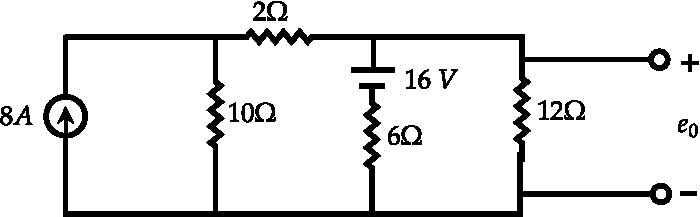
\includegraphics[height=2cm,width=6cm]{E-A-13}
		\caption{}
		\label{}
	\end{figure}
	 \begin{tasks}(2)
		\task[\textbf{a.}]48V
		\task[\textbf{b.}]24V
		\task[\textbf{c.}]36V
		\task[\textbf{d.}]28V
	\end{tasks}
	\item In the circuit of figure, the value of the voltage source $E$ is
	\begin{figure}[H]
		\centering
		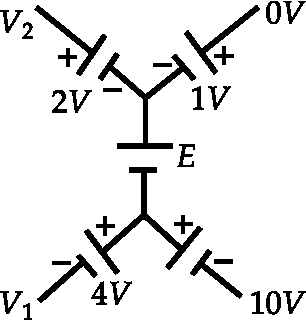
\includegraphics[height=3cm,width=3cm]{E-A-14}
		\caption{}
		\label{}
	\end{figure}
	 \begin{tasks}(2)
		\task[\textbf{a.}]$-16 \mathrm{~V}$
		\task[\textbf{b.}]$4 \mathrm{~V}$
		\task[\textbf{c.}] $-6 V$
		\task[\textbf{d.}]  $16 \mathrm{~V}$
	\end{tasks}
	\item The voltage $\mathrm{V}$ in figure is equal to:
	\begin{figure}[H]
		\centering
		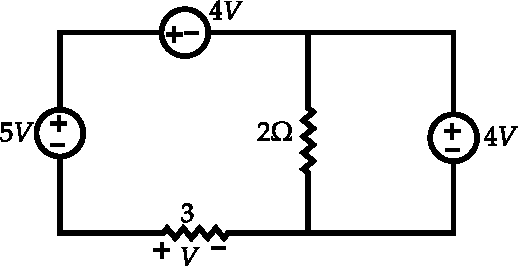
\includegraphics[height=2.5cm,width=5cm]{E-A-15}
		\caption{}
		\label{}
	\end{figure}
	 \begin{tasks}(2)
		\task[\textbf{a.}]$3 \mathrm{~V}$
		\task[\textbf{b.}]$-3 \mathrm{~V}$
		\task[\textbf{c.}]$5 \mathrm{~V}$
		\task[\textbf{d.}]None of these 
	\end{tasks}
	\item The voltage in figure is
	\begin{figure}[H]
		\centering
		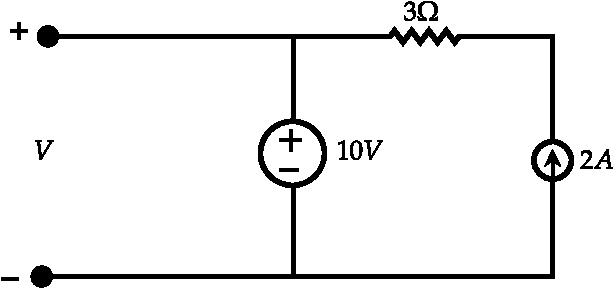
\includegraphics[height=2.5cm,width=5cm]{E-A-16}
		\caption{}
		\label{}
	\end{figure}
	 \begin{tasks}(2)
		\task[\textbf{a.}]$10 \mathrm{~V}$
		\task[\textbf{b.}]$15 \mathrm{~V}$
		\task[\textbf{c.}]$5 \mathrm{~V}$
		\task[\textbf{d.}]None of these 
	\end{tasks}
\item What is the value of $R$ required for maximum power transfer in network shown above?
\begin{figure}[H]
	\centering
	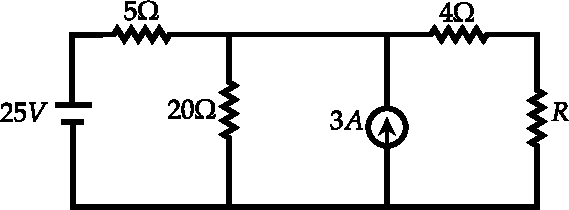
\includegraphics[height=2cm,width=5cm]{E-A-17}
	\caption{}
	\label{}
\end{figure}
 \begin{tasks}(2)
	\task[\textbf{a.}]$2\Omega$
	\task[\textbf{b.}]$4\Omega$
	\task[\textbf{c.}]$8\Omega$
	\task[\textbf{d.}]$16\Omega$
\end{tasks}
\item The voltage across the terminal $a$ and $b$ in figure is:
\begin{figure}[H]
	\centering
	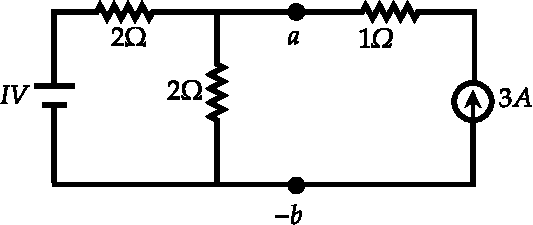
\includegraphics[height=2.2cm,width=5cm]{E-A-18}
	\caption{}
	\label{}
\end{figure}
 \begin{tasks}(2)
	\task[\textbf{a.}]$0.5 \mathrm{~V}$
	\task[\textbf{b.}]$3.0 \mathrm{~V}$
	\task[\textbf{c.}]$3.5 \mathrm{~V}$
	\task[\textbf{d.}]$4.0 \mathrm{~V}$ 
\end{tasks}
\item The nodal method of circuit analysis is based on
 \begin{tasks}(2)
	\task[\textbf{a.}]KVL and ohm's law
	\task[\textbf{b.}]KCL and Ohm's law
	\task[\textbf{c.}]$\mathrm{KCL}$ and $\mathrm{KVL}$
	\task[\textbf{d.}]KCL, KVL and Ohm's law 
\end{tasks}
\item The current $i_{4}$ in the current of figure is equal to:
\begin{figure}[H]
	\centering
	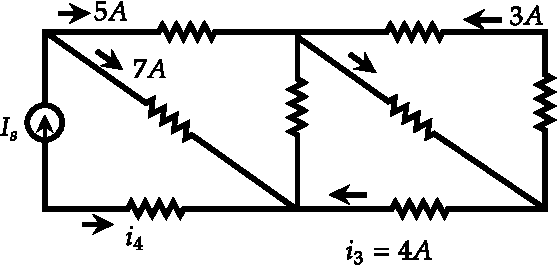
\includegraphics[height=2.8cm,width=5.cm]{E-A-19}
	\caption{}
	\label{}
\end{figure}
 \begin{tasks}(2)
	\task[\textbf{a.}]$12 \mathrm{~A}$
	\task[\textbf{b.}]$-12 \mathrm{~A}$
	\task[\textbf{c.}]$4 \mathrm{~A}$
	\task[\textbf{d.}]None of these
\end{tasks}
\item Thevenin equivalent voltage $V_{\mathrm{AB}}$ and resistance $\mathrm{R}_{\mathrm{Th}}$ across the terminals $\mathrm{AB}$ in the above circuit are
\begin{figure}[H]
	\centering
	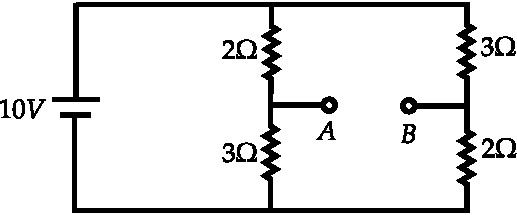
\includegraphics[height=2.5cm,width=5cm]{E-A-20}
	\caption{}
	\label{}
\end{figure}
 \begin{tasks}(2)
	\task[\textbf{a.}]$6 \mathrm{~V}, 5 \Omega$
	\task[\textbf{b.}]$4 \mathrm{~V}, 5 \Omega$
	\task[\textbf{c.}]$2 \mathrm{~V}, 2.4 \Omega$
	\task[\textbf{d.}]$2 \mathrm{~V}, 2.5 \Omega$
\end{tasks}
\item The differential equation for the current $i(t)$ in the circuit of the figure is
\begin{figure}[H]
	\centering
	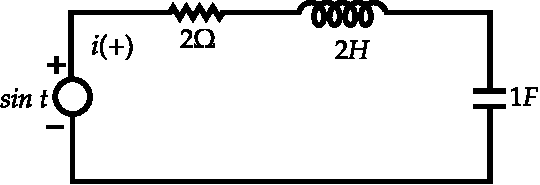
\includegraphics[height=2cm,width=5cm]{E-A-21}
	\caption{}
	\label{}
\end{figure}
 \begin{tasks}(2)
	\task[\textbf{a.}] $2 \frac{d^{2} i}{d t^{2}}+2 \frac{d i}{d t}+i(t)=\sin t$
	\task[\textbf{b.}]$\frac{d^{2} i}{d t^{2}}+2 \frac{d i}{d t}+2 i(t)=\cos t$
	\task[\textbf{c.}]$2 \frac{d^{2} i}{d t^{2}}+2 \frac{d i}{d t}+i(t)=\cos t$
	\task[\textbf{d.}] $\frac{d^{2} i}{d t^{2}}+2 \frac{d i}{d t}+2 i(t)=\sin t$
\end{tasks}
\item The $R C$ circuit shown in the figure is
\begin{figure}[H]
	\centering
	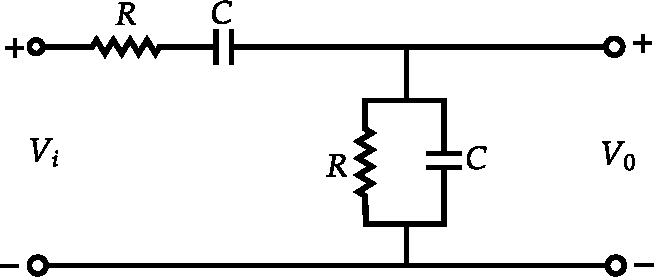
\includegraphics[height=2.5cm,width=5cm]{E-A-22}
	\caption{}
	\label{}
\end{figure}
 \begin{tasks}(2)
	\task[\textbf{a.}]a low-pass filter
	\task[\textbf{b.}]a high-pass filter
	\task[\textbf{c.}]a band-pass filter
	\task[\textbf{d.}]a band-regeat filter 
\end{tasks}
\item In the circuit shown below, the value of $R_{L}$ such that the power transferred to $R_{L}$ is maximum.
\begin{figure}[H]
	\centering
	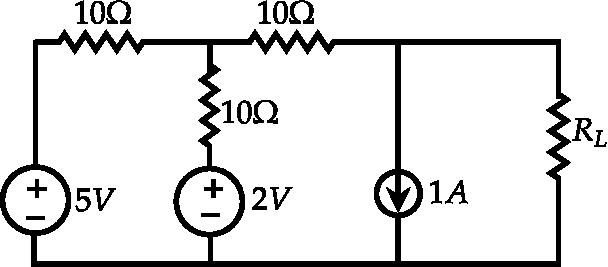
\includegraphics[height=2.3cm,width=5cm]{E-A-23}
	\caption{}
	\label{}
\end{figure}
 \begin{tasks}(2)
	\task[\textbf{a.}]$5\Omega$
	\task[\textbf{b.}]$10\Omega$
	\task[\textbf{c.}]$15\Omega$
	\task[\textbf{d.}]$20\Omega$
\end{tasks}
\item Find the value of $C$ to deliver the maximum power to load.
\begin{figure}[H]
	\centering
	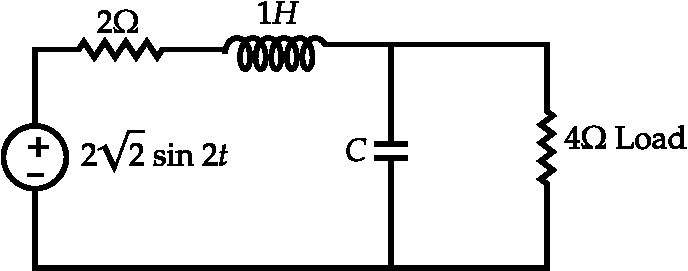
\includegraphics[height=2.3cm,width=5.2cm]{E-A-24}
	\caption{}
	\label{}
\end{figure}
 \begin{tasks}(2)
	\task[\textbf{a.}] $0.125 \mathrm{~F}$
	\task[\textbf{b.}] $0.5 \mathrm{~F}$
	\task[\textbf{c.}]$2 \mathrm{~F}$
	\task[\textbf{d.}] 4
\end{tasks}
\item Find $Z_{L}$ such that maximum power is transferred to it.
\begin{figure}[H]
	\centering
	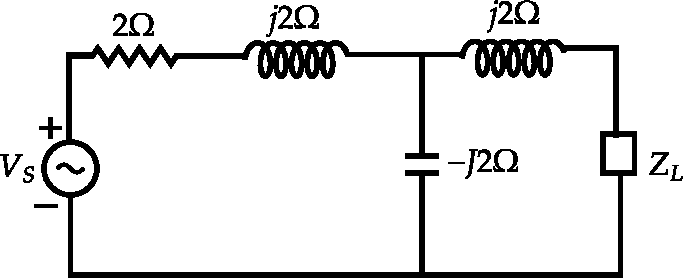
\includegraphics[height=2.5cm,width=5.4cm]{E-A-25}
	\caption{}
	\label{}
\end{figure}
 \begin{tasks}(2)
	\task[\textbf{a.}]$(2+\dot{J} 2) \Omega$
	\task[\textbf{b.}] $(2-j 2) \Omega$
	\task[\textbf{c.}]$(-J 2 \Omega)$
	\task[\textbf{d.}] $2 \Omega$
\end{tasks}
\item The voltage across a capacitor is triangular in waveform. The waveform of current is
 \begin{tasks}(2)
	\task[\textbf{a.}]triangular
	\task[\textbf{b.}]trapezoidal
	\task[\textbf{c.}]Sinusoidal
	\task[\textbf{d.}] Rectangular 
\end{tasks}
\item The value of $R_{\text {in }}$ of the network
\begin{figure}[H]
	\centering
	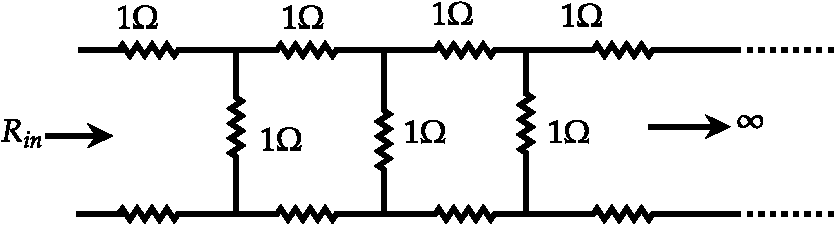
\includegraphics[height=2.2cm,width=7cm]{E-A-26}
	\caption{}
	\label{}
\end{figure}
 \begin{tasks}(2)
	\task[\textbf{a.}]$1.62 \Omega$
	\task[\textbf{b.}]$2 \Omega$
	\task[\textbf{c.}]$\frac{1}{3} \Omega$
	\task[\textbf{d.}]$\frac{1}{2} \Omega$
\end{tasks}
\item The maximum power that can be distributed in the load in the circuit shown is
\begin{figure}[H]
	\centering
	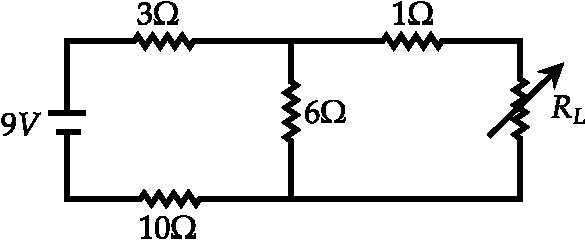
\includegraphics[height=2.3cm,width=5.3cm]{E-A-27}
	\caption{}
	\label{}
\end{figure}
 \begin{tasks}(2)
	\task[\textbf{a.}]$0.396 \mathrm{~W}$
	\task[\textbf{b.}]$6 \mathrm{~W}$
	\task[\textbf{c.}]$6.75 \mathrm{~W}$
	\task[\textbf{d.}]$13.5 \mathrm{~W}$ 
\end{tasks}
\item If $\mathrm{V}_{\mathrm{c}}(\mathrm{f})=4 \cos \left(10^{5} \mathrm{t}\right) \mathrm{V}$ in the circuit, find $\mathrm{Vs}$.
\begin{figure}[H]
	\centering
	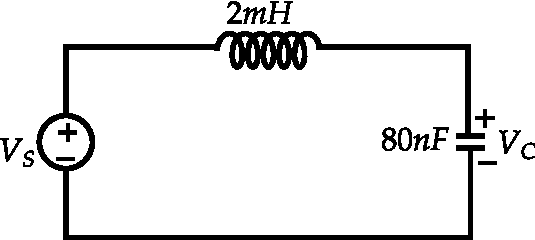
\includegraphics[height=2.2cm,width=5cm]{E-A-28}
	\caption{}
	\label{}
\end{figure}
 \begin{tasks}(2)
	\task[\textbf{a.}]$-6.4 \cos 10^{5} \mathrm{t} \mathrm{V}$
	\task[\textbf{b.}]$2.4 \cos 10^{5} \mathrm{t} \mathrm{V}$
	\task[\textbf{c.}]$6.4 \cos 10^{5} \mathrm{t} \mathrm{V}$
	\task[\textbf{d.}]$-2.4 \cos 10^{5} \mathrm{t} \mathrm{V}$ 
\end{tasks}
\item Determine the current through the branch $\mathrm{AB}$ of network shown below.
\begin{figure}[H]
	\centering
	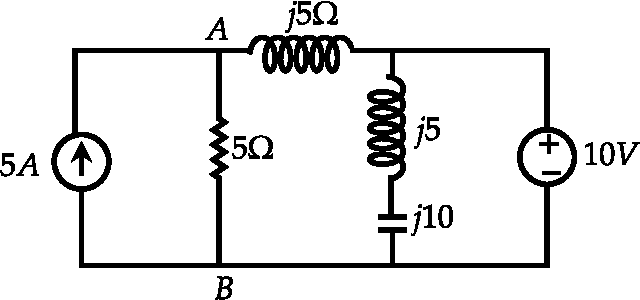
\includegraphics[height=2.8cm,width=5.3cm]{E-A-29}
	\caption{}
	\label{}
\end{figure}
 \begin{tasks}(2)
	\task[\textbf{a.}]$3.5+\dot{\mathrm{J}} 1.5$
	\task[\textbf{b.}]$3.5-\dot{J} 1.5$
	\task[\textbf{c.}]$1.5+\dot{J} 3.5$
	\task[\textbf{d.}]$1.5-\dot{J} 3.5$ 
\end{tasks}
\item What is the ratio of currents in the circuit due to $3 \mathrm{~A}$ and $2 \mathrm{~A}$ source? Current is taken through $\mathrm{R}$.
\begin{figure}[H]
	\centering
	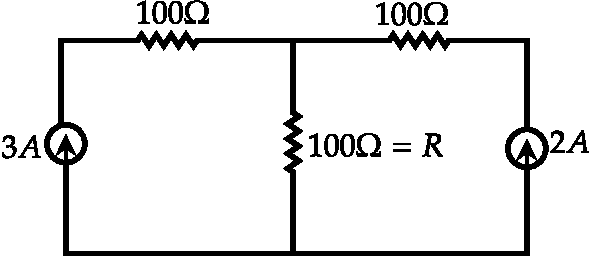
\includegraphics[height=2.2cm,width=5cm]{E-A-30}
	\caption{}
	\label{}
\end{figure}
 \begin{tasks}(2)
	\task[\textbf{a.}]$\frac{3}{2}$
	\task[\textbf{b.}]$\frac{2}{3}$
	\task[\textbf{c.}]$\frac{9}{4}$
	\task[\textbf{d.}] $\frac{4}{9}$ 
\end{tasks}
\end{enumerate}